% --------------------------------------------------------------------------- %
%      _ _                        _
%   __| (_)___  ___ _   _ ___ ___(_) ___  _ __
%  / _` | / __|/ __| | | / __/ __| |/ _ \| '_ \
% | (_| | \__ \ (__| |_| \__ \__ \ | (_) | | | |
%  \__,_|_|___/\___|\__,_|___/___/_|\___/|_| |_|
% --------------------------------------------------------------------------- %
\chapter{Examining Sound ARt Experiences}
\label{sec: discussion}
\epigraph{\emph{Alice has stepped through the looking glass [...] It is the job all future artists and activists to use this technology for the better, to bring people together, and uproot social injustice.}}{\citep[]{skwarek2018}}

\begin{figure}
    \centering
    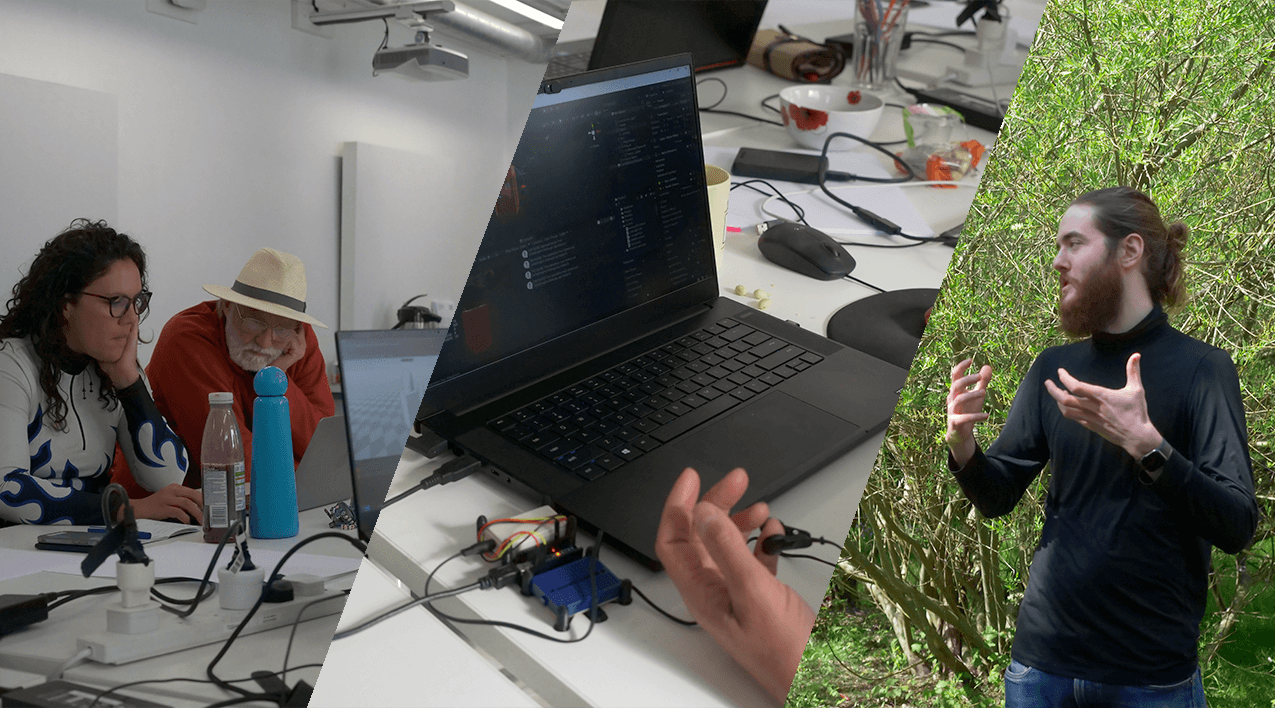
\includegraphics[width=1\linewidth]{08-discussion/chapter-fig.png}
    \captionsetup{labelformat=empty}
    \caption[Participants experiencing and demonstrating usage of Project North Star (own photographs)]{}
\end{figure}

\clearpage
% --------------------------------------------------------------------------- %
\section{Summary}\label{sec: discussion-summary}
In this chapter I aim to bring together the results of the past three study chapters, and discuss the implications they may have on what could be termed the sonic medium of \gls{ar}. It is separated into three sections. In the first, I review the steps taken so far in the thesis that have allowed space for a unique positionality when considering the potential for \gls{ar} as a medium for sound-driven art works. In the second, I outline the methodology that lead to the sound \gls{art} that makes up my practice-based research. In the third section, the combined results of the previous three chapters are discussed in the context of materiality, embodiment, and space; resurfacing and re-introducing the theories explored in \autoref{sec: theory}.
% --------------------------------------------------------------------------- %
\section{From Overlay to Instrument}\label{sec: discussion-review}
In \autoref{sec: introduction}, I outlined my motivations for asking the following questions, which were addressed in \autoref{sec: review} and \autoref{sec: theory}: 

\begin{itemize}
    \RQgenealogy
    \RQtheory
\end{itemize}

The present thesis began in \autoref{sec: review} with an exploration of the landscape of historical and contemporary \gls{ar} research and development spanning the past thirty years. Common forms, such as headset-, handheld- and projective-based \gls{ar} were outlined, as well as typical sensory displays, allowing interaction and feedback with the visual, auditory, touch-based, and smell and taste senses. Furthermore, the processes by which \gls{ar} mediates reality were laid out using Schraffenberger's categorisation of relationships and \gls{ar} subforms: augmented, diminished, altered, and hybrid reality, as well as extended perception \citep{schraffenberger2018}. Despite this wealth of possible avenues for \gls{ar} experience composition, the paradigmatic form of \gls{ar} we hear about or see are predominantly characterised by being \textit{visual displays that overlay information}. Thus far in the thesis, this has been referred to as ocularcentric layering paradigm, or typical \gls{ar}. This can be explained by a number of phenomena, but examining the origination of \gls{ar} in the \gls{mic} by way of U.S. Defence funding, it is not a surprise. This has had a compounded effect on the forms that \gls{ar} finds itself being co-opted for in the arts. Several creative and expressive works were explored, that engaged in \gls{ar} because of its ability to sensorily engage participants, induce rich aesthetic experience, enable collaborative expression, and empower new forms of agency and activism. Nonetheless, there are but a few examples of sound art \gls{ar} experiences in comparison to visual counterparts because of the typical form of \gls{ar}.

In proposing the development of \gls{ar} as a medium for the creation of immersive sound artworks, its use as an instrument, or tool for sound art installation, I drew on several areas of importance in \autoref{sec: theory}, first aesthetic experience and the `4E's', and then materiality, embodiment, and space. It began with a grounding in the concept of 'art as experience', drawing from the work of \citep{dewey1934}. Dewey states that the capitalistic reverence of fine art, notably by the `nouveau riches', has led to art being put on a pedestal - disconnecting it from its origin and operation in the everyday experiences of people. Leddy and Puolakka have since proposed that `material of art should be from all sources and art should be accessible to all' \citeyearpar{leddy2021}. Dewey points towards the aesthetic experience that art entails, and notes that the `live creature' is inseparable from the environment in which they are embedded. Today, despite social media as a platform for cultural production of artistic works having some merits, the fabric on which it is built is no different from the capitalist mechanisms that separated art from experience in the first place. Thus, \glshyperlink[open-source]{opensource}, hacker, \gls{diy}, and maker approaches were proposed as a method of democratising `all sources' of art, and attempting to increase accessibility. The focus on the body by Dewey also points out the move towards tangible interface development, participatory design, and human-centred design that were outlined in \autoref{sec: method-resistance-maker}. To delve deeper into this experience of art, I proposed an enactivist approach to considering cognition in experience. Often called \gls{4ec}, it states that cognitive process are embodied, embedded, enactive, and extended \citep{gallagher2017}. In considering the design, performance, and experience of \gls{ar}, \gls{4ec} offers a fresh perspective on concepts such as agency, action, perception, immersion, and spatial engagement.

The first theoretical lens through which to examine \gls{ar}'s design in computational art and music practice involved outlined the importance of a complex systems framing of interface use and performance. I drew on existing research from the field of digital musical instrument design \citep{magnusson2009a,discipio2003,essl2006,armstrong2006,hayes2019,chevalier2018} in order to demonstrate the usefulness of considering the material of performance systems as complex, and ecosystemic. To examine what happens in the experience of participants, the second lens was one that took seriously the assertions of \gls{4ec}, namely that cognitive processes in experience are embodied, embedded, enactive and extended. I draw from multiple disciplines of similar theoretical and practical work in \gls{vr} and \gls{ar} to show how \gls{4ec} offers a novel framing by which to consider the experience of \gls{ar} by participants, audiences, and performers. Closing out the trio of theoretical lenses, is a grounding of the aforementioned consequence of \gls{ar} for the experience and construction of `space'. I first critically examine the term `Metaverse' \citep{stephenson1992}. Its modern-day origin is in technologies like \gls{ar} and \gls{vr}, which in turn sprung from` deep within the military and Western - scientific - industrial - patriarchal complex' \citep{davies2004}, and its current operation has been heavily co-opted by cryptocurrency projects. Because of this, in its current state, the `Metaverse' is hardly fertile ground for the `live creature' to experience art `accessibly', and from `all sources' \citep{dewey1934,leddy2021}, indeed, it mirrors the exact profit and exploitation motive of the historical context it originated in.



% --------------------------------------------------------------------------- %
\section{Engaging in a DIY Approach to Sound ARt}\label{sec: discussion-method}
A clear positionality from within the arts, one that stands in contrast with the militaristic and industrial applications and their effect on the typical form of \gls{ar} technologies was outlined in \autoref{sec: method}. This chapter proposed methodological approach to compose, iterate, and perform sound \gls{art} that would allow the addressing of the following research questions through practical contributions to the field of interactive music systems: 

\begin{enumerate}
    \RQmedium
    \RQexperience
    \RQfuture
\end{enumerate}

This began with the explication of the concept of resistance, and its importance in my rationale for choosing specific methods. Specifically, I highlighted the role of \gls{ar}'s paradigmatic form as a closed-source consumer technology, as a visual technology, and, and as a medium that overlays information, as primary motivators and areas for change in the field. In practice, this approach led to the evaluation of three aesthetically, functionally, and methodologically distinct interactive music systems over the course of the thesis, \textit{\nameref{sec: area} (2020)}, \textit{\nameref{sec: polaris} (2021)}, and \textit{\nameref{sec: polygons} (2022)}. These experiences, or sound \gls{art}works were developed using a set of design guidelines that were iterated on over the course of the thesis, and will be outlined in \autoref{sec: discussion-guidelines}. 

There are clear limitations to the the generalisability of specific findings in the \gls{ar} experiences developed. Having to adapt to the COVID-19 pandemic meant developing methods that revolved more around autoethnographic / autobiographical study of the systems. This, while potentially offering more depth of insight over long-term deployment of \textit{area\textasciitilde{}} for example, don't provide the kind of breadth of insight that the participant studies in \textit{polaris\textasciitilde{}} did for example. Qualitative analysis, while conducted with rigour throughout the thesis, still only speaks from a position that highlights the subjectivity of participant experience, and specificities of the experience being examined. There are, as always, positives and negatives to this. While providing considerable retrospective insight into my own creative practice, and providing the groundwork for developing the theoretical propositions in the next section, and patterns in \autoref{sec: discussion-guidelines}: \nameref{sec: discussion-guidelines}, they do not provide any objective and generalisable results about the nature of experience or reality. Perhaps there is no such thing, and the immense diversity of possible \gls{ar} experience serves to demonstrate this. Another benefit of the research methods involved in this approach is their propensity to provoke and generate questions, which have surfaced throughout this thesis.



% --------------------------------------------------------------------------- %
\section{Combined Results: \textit{area\textasciitilde{}}, \textit{polaris\textasciitilde{}}, and \textit{polygons\textasciitilde{}}}\label{sec: discussion-medium}

The previous three chapters outlined the experiences, compositions, performances, and results of engaging with \gls{ar} as a medium for sound \gls{art} production. In this section I would like to briefly touch on the findings from each.

\subsection{\textit{area\textasciitilde{}}}
\textit{area\textasciitilde{}}, which could be classified as a pilot study, or a research probe into the possibilities of non-visual \gls{ar} experience, uncovered the following results from an \gls{abd} research method. Firstly that the blending of \textit{real and virtual auditory environments} resulted aesthetically in the creation of a third, augmented environment that was greater in experiential nature than the sum of its parts (not simply a combinatorial layering). Secondly, the ability to spectromorphologically manipulate sounds in real-time in this augmented environment with the body proved an engaging compositional tool. Lastly, the potential for creating believable illusions of real-world sound sources from these manipulated and spatialised virtual sounds was highlighted.

\subsection{\textit{polaris\textasciitilde{}}}
\textit{polaris\textasciitilde{}}, the audio-visual piece created for the \gls{pns} headset using Unity and PureData engaged participants fruitfully, with many noting their ability to express themselves audiovisually in creative ways. The focus for \textit{polaris\textasciitilde{}} was primarily on the ability to create this type of experience in a cost-effective, and privacy respecting way. Evaluation of the piece was provided through the experiential testing of ten participants, and the grounded-theory analysis of their interview transcripts. While the analysis was not, on its own, sufficient to draw conclusive guidelines for design, or objective facts about the efficacy of the experience, it did shed light on several connections between elements of this specific experience: learning, comfort, safety, spatial perception, visual-, sonic-, and action-led immersion, and physicality of virtual content.

\subsection{\textit{polygons\textasciitilde{}}}
\textit{polygons\textasciitilde{}}, the last of the experiences, could be described as a first look (or listen) into the implications of sound \gls{art} performances. For me, it provided a new, visceral type of embodied performance and led to a kind of `technologically mediated dialogue between hybrid self and hybrid environment', which in itself demonstrated the delicate balance of technological agency and sense of `uncontrol'. It provided me with the resulting questions: 
\begin{itemize}
    \item Can we avoid `spectacle' of \gls{ar}? How else can we meaningfully engage audiences who are new to \gls{ar}?
    \item How can we invite the audience into \gls{ar} musical performance more effectively?
    \item Is wearing more technology necessarily the best avenue for a focus on embodied performance?
    \item What would an \gls{ar} ensemble look, sound, and feel like for both performer and audience?
    \item Could \gls{ar} be appropriated for real-time networked performance of physically separate spaces?
\end{itemize}

% --------------------------------------------------------------------------- %
\section{Design Guidelines for Sound ARt}\label{sec: discussion-guidelines}
In \autoref{sec: method}, I outlined the primary vehicle through which to address the key topics and questions of the thesis: the creation and evaluation of sound \gls{art} experiences. These have, in their development and iteration, drawn on a proto-framework of implicit designerly tendencies or `guidelines' that I have found effective - drawing from points of resistance (\autoref{sec: method-resistance}), and relevant perspectives from the field (\autoref{sec: theory}). In this section the aim is to outline these guidelines in a way that may allow for the creation of similar works of \gls{art} in the future, by members of the experimental music, computational art, and digital humanities fields. 

\begin{figure}
    \centering
    {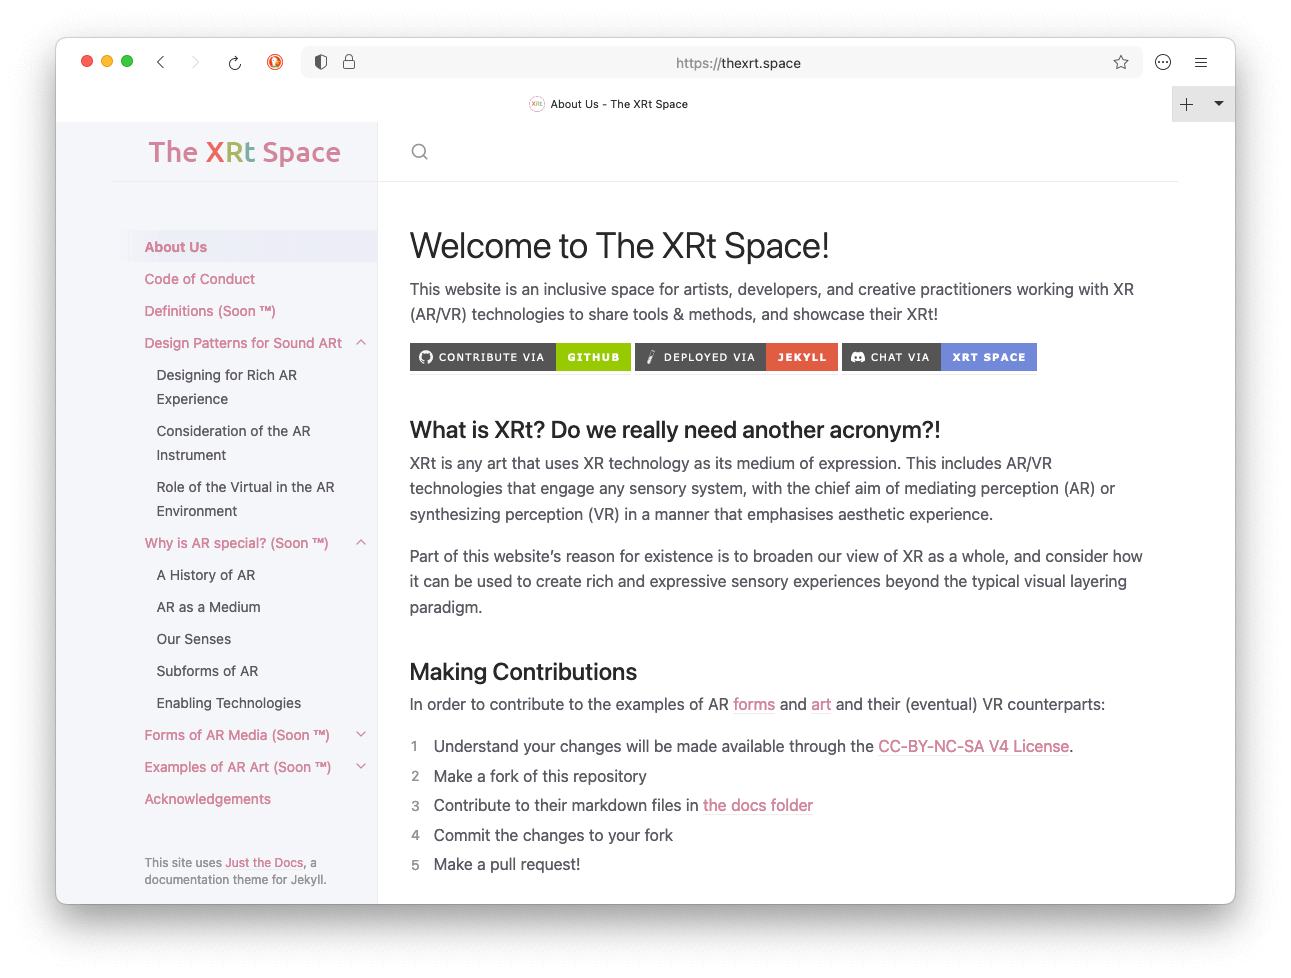
\includegraphics[width=.75\linewidth]{08-discussion/thexrtspace.png}}
    \caption[The XRt Space website]{The XRt Space website}
\end{figure}\label{fig: thexrtspace}

These design guidelines are therefore subject to iteration, and the latest version can be found on \href{https://sambilbow.github.io/thexrtspace}{the XRt Space website} (\autoref{fig: thexrtspace}), a community-editable repository created to host and update them. The principles used to guide the patterns draw on the resistances outlined in \autoref{sec: method-resistance}, namely taking a \gls{diy} approach, decoupling from the ocularcentric and layering paradigms of typical \gls{ar} experience, and attempting to navigate an inherently consumerist space whilst trying not to contribute to exploitative systems of oppression that uphold it. They are also guided by the theoretical lenses of \autoref{sec: theory} and propositions of \autoref{sec: conclusion}: which states that a participant's and performer's cognitive processes in the experience of \gls{ar} artworks are embodied, embedded, enacted, and extended, and have the potential to be modulated to extents that offer novel aesthetic experiences of augmented \hyperref[sec: discussion-medium-material]{materiality}, \hyperref[sec: discussion-medium-embodiment]{embodiment}, and \hyperref[sec: discussion-medium-space]{space}. The following sections outline three design guidelines, \textit{\nameref*{sec: discussion-guidelines-experience}}, \textit{\nameref*{sec: discussion-guidelines-instrument}}, and \textit{\nameref*{sec: discussion-guidelines-environment}}.

\subsection{Designing for Rich AR Experience}\label{sec: discussion-guidelines-experience} 
\autoref{sec: theory} drew on a number of theoretical propositions, and put forward that \gls{ar} has the potential to scaffold new modes of performance and expression in the arts and music, furthermore, that from an enactivist approach experience, this would consist in radically modulating the material, embodied, and spatial experience of participants. This is the starting point for ideating and designing an artistic \gls{ar} experience in the present thesis. This pattern addresses the issue of the typicality of \gls{ar} experience being simple interactions with visual overlay devices. It approaches experience ideation from a holistic and multisensory, or `modalities-encompassing' \citep{schraffenberger2018} perspective. Furthermore, the \glshyperlink[`4Es' of an enactivist approach]{4ec} can be considered as conditions for what could be described as immersive and `rich experience' \citep{bilbow2021}. As highlighted in \autoref{sec: theory-materiality}, enactivist principles have been offered as guidelines for the creation of interactive systems in the past; Essl and O'Modhrain \citeyearpar{essl2006}, Armstrong \citeyearpar{armstrong2006}, and Hayes \citeyearpar{hayes2019} suggest this approach in the design of new musical instruments. 

The concept of rich experience also stands in stark contrast to the current direction of corporate \gls{xr} technologies, where it is being developed to \textbf{replace} in-person interactions e.g. by facilitating in-headset `work from home' \glspl{ve} such as Meta Horizons. It also stands in contrast with the marketed push towards \gls{ar} as a tool for driving commerce through targeted advertisements. How as artists and musicians can we avoid the corporate, commercial, ocularcentric, and overlay approach to \gls{ar}? How can we offset the dystopian hell-scape, painted by designer and film-maker Keiichi Matusda in various film shorts (see \autoref{fig: discussion-matsuda}).

\begin{figure}[hbt]
    \centering
    \captionsetup{justification=centering}
    \subcaptionbox{\textit{`The Pusher / The Entertainment'} \citep[from][]{matsuda2009}}[.45\linewidth]{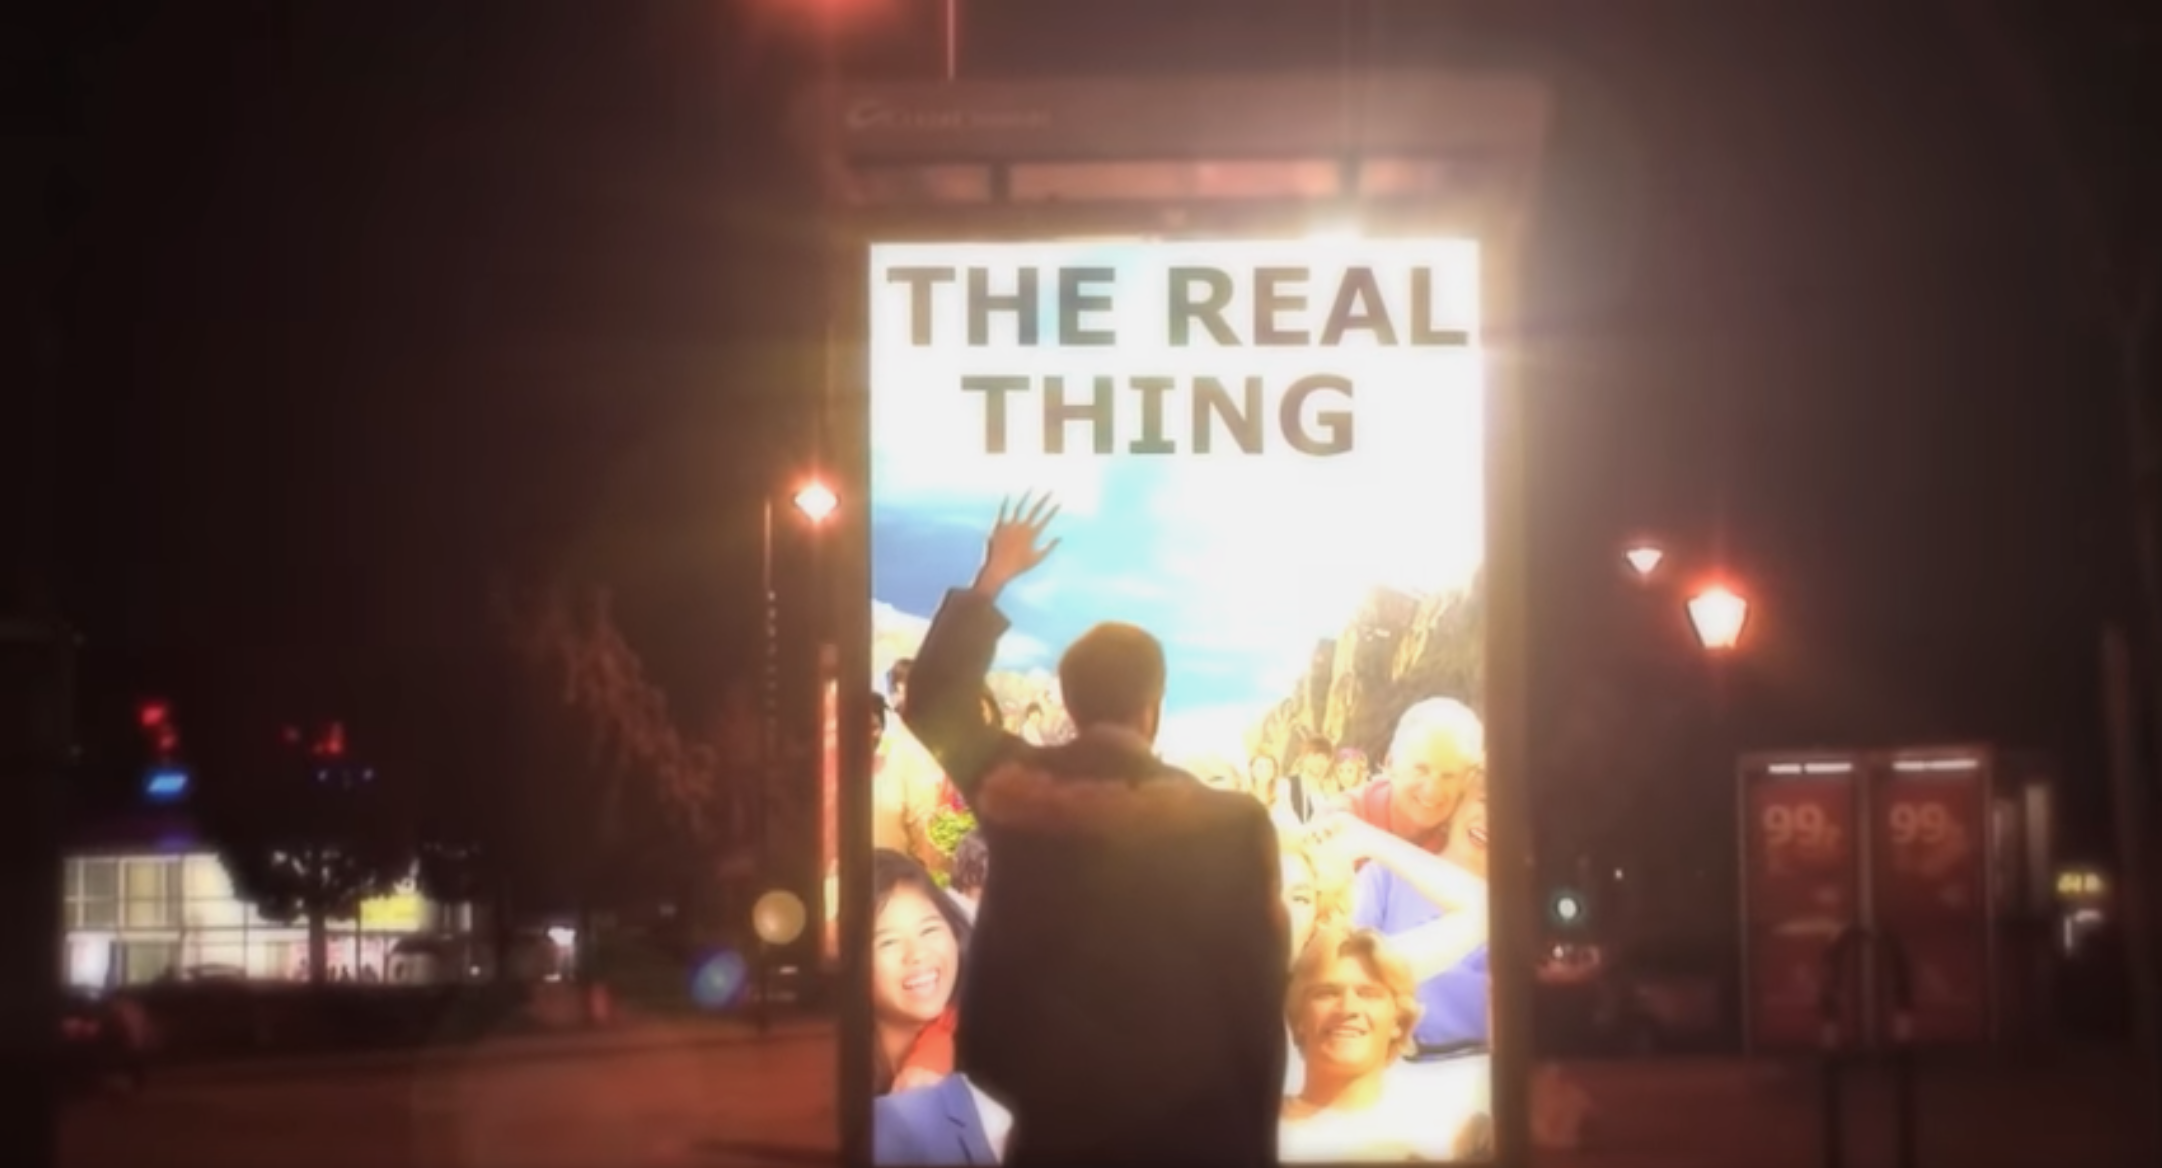
\includegraphics[height=3.8cm]{08-discussion/matsuda2009.png}}
    \hfill
    \subcaptionbox{\textit{`Augmented (hyper)Reality: Domestic Robocop'} \citep[from][]{matsuda2010}}[.45\linewidth]{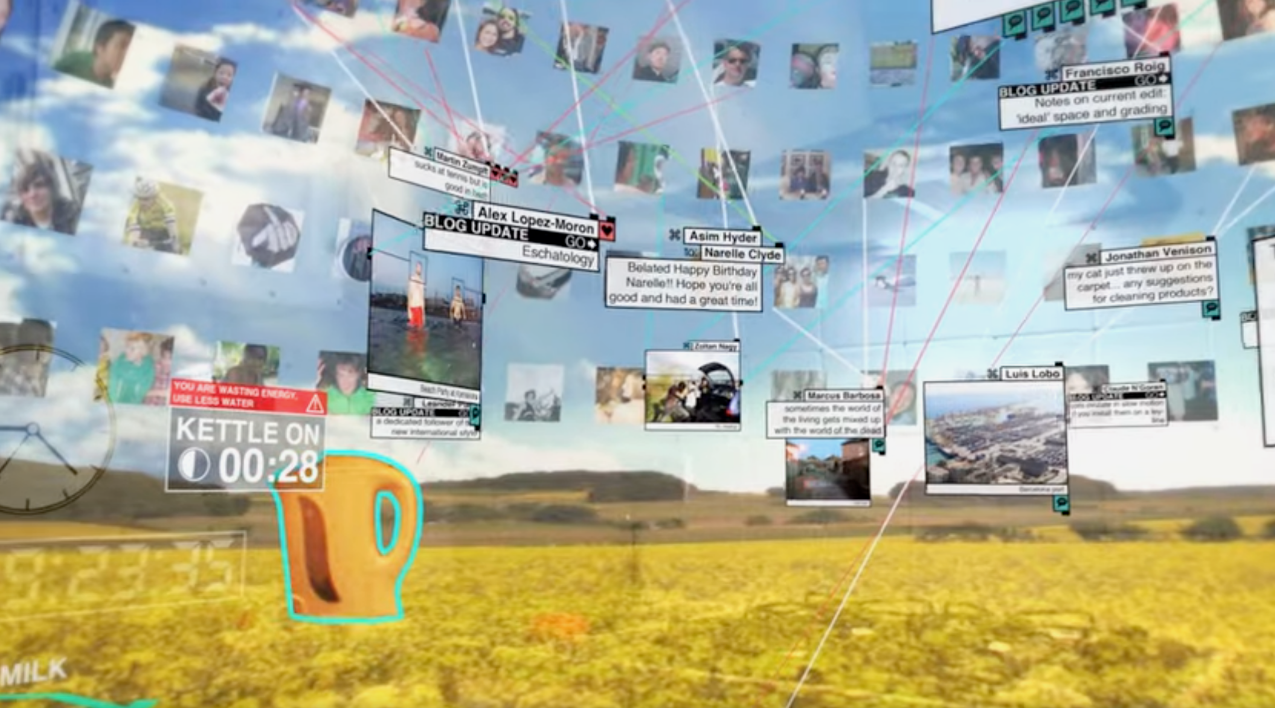
\includegraphics[height=3.8cm]{08-discussion/matsuda2010.png}} \\
    \vspace{0.5cm}
    \subcaptionbox{\textit{`HYPER-REALITY'} \citep[from][]{matsuda2016}}[.45\linewidth]{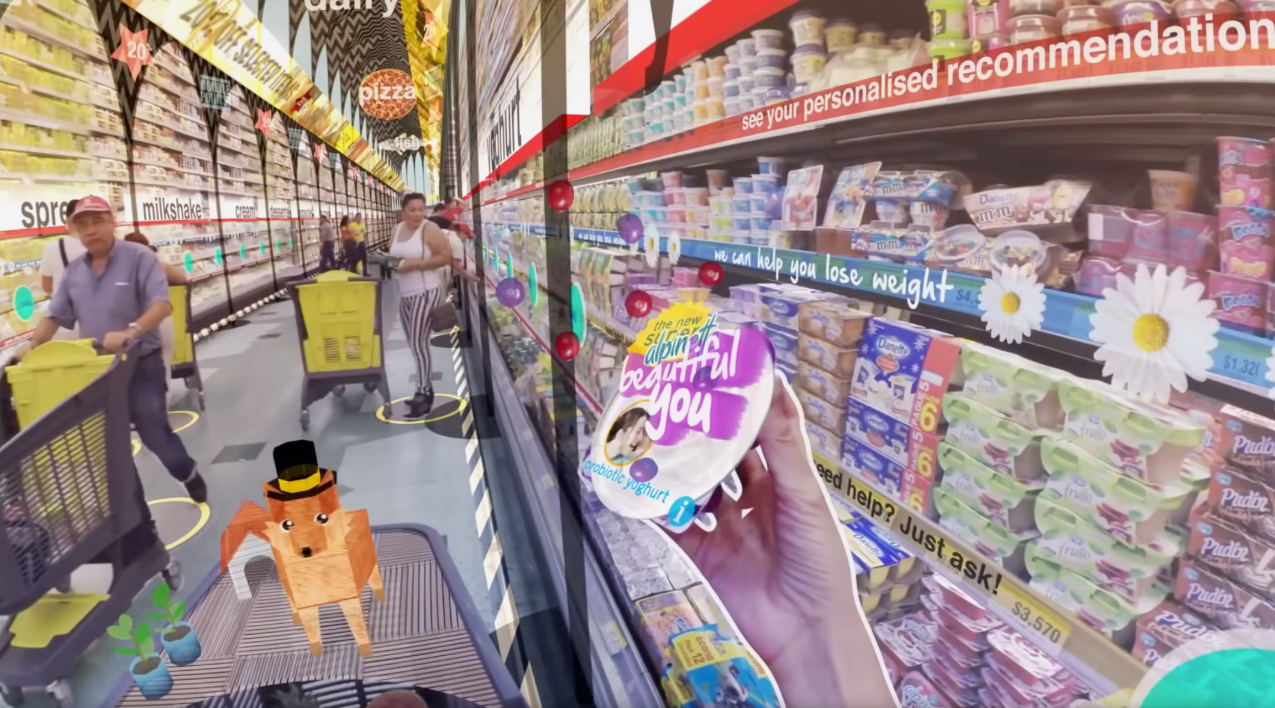
\includegraphics[height=3.8cm]{08-discussion/matsuda2016.png}}
    \hfill
    \subcaptionbox{\textit{`Merger'} \citep[from][]{matsuda2019}}[.45\linewidth]{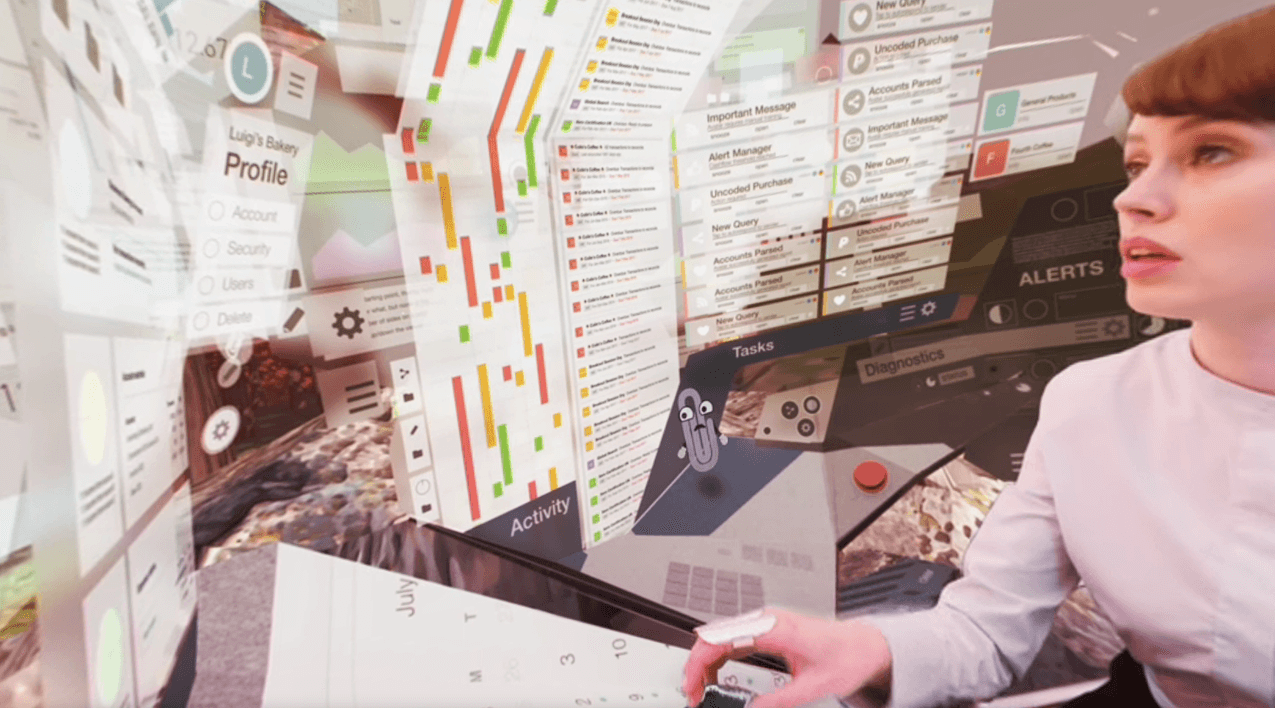
\includegraphics[height=3.8cm]{08-discussion/matsuda2019.png}}
    \caption{Keiichi Matusda's short films on dystopian AR futures}
    \label{fig: discussion-matsuda}
\end{figure}

\subsubsection{Centre the experience on two or more sensory interactions}
Whether it is Dewey's concept of the `live creature', or the contemporary enactivist's framing of the importance of embodiment, the \gls{ar} experience ought to be \textit{centred on two or more sensory interactions}. It may include any combination of sensory interaction (display or sensing) types, e.g. visual (vision), auditory (hearing), vestibular (movement and balance), olfactory (smell), gustatory (taste), and somatosensory (touch). This ensures grounding in the importance of the participants agency and sensorimotor structure. Here, the importance of considering the \gls{ar} experience as an enaction, rather than an abstract internal representation that they are thinking and then acting upon is crucial.

\subsubsection{Invoke a meaningful relationship between the real and virtual}
\gls{ar}'s medium specificity, discussed in \autoref{sec: discussion-medium-material}, should be at the forefront of intentional design choices. If, as it will come to be argued, \gls{ar} is unique because of its `invocation of relationships between real and virtual processes in the axes of spatial, thematic, material and ecological distance', these relationships become a key handle by which artists and musicians can \textit{meaningfully steer experience to achieve aesthetic experiences}. Consider the following:
\begin{itemize}
    \item Spatial: to what extent should the virtual and real be spatially aligned or even spatially related?
    \item Thematic: to what extent should the virtual and real be thematically similar, what effect might this have on participants' sense of sensory congruency if distant instead?
    \item Material: to what extent should the virtual be materially similar to the real environment in which \gls{ar} brings it into conversation with? 
    \item Ecological: to what extent should the virtual act as part of the real environment, how does this suit the overall narrative intention of the piece?
\end{itemize}
For the artist or musician, the interest and specificity of \gls{ar} might lend itself to tending towards the revealing the differences rather than the similarities between the virtual and the real!

\subsubsection{Implement an AR subform}
In considering the embodied experience of participants, employ Schraffenberger's taxonomy of \gls{ar} subforms. As discussed in \autoref{sec: discussion-medium-embodiment}, augmented embodiment is achieved through the fact that \gls{ar} has the potential to radically modulate a participants sense of self, other, and environment. The present thesis has made a clear standpoint on the role of the \gls{mic} in biasing the development and conceptualisation of \gls{ar} towards that of an overlay device or heads-up display. Artists and musicians engaging in \gls{ar} will already be tending towards the altered and hybridised subforms of \gls{ar} rather than the purely augmenting; but it is worth mentioning here that significant improvements in the effectiveness of \gls{ar} in delivering aesthetic experience lies in considering the \textit{process} (see subform) by which perception is mediated by \gls{ar}.

\subsection{Consideration of the AR Instrument}\label{sec: discussion-guidelines-instrument}
When describing the means through which a participant or performer meaningfully interacts or engages in any kind of information transfer in the \gls{ar} system, it is through what could be termed the \gls{ar} Instrument. The following categorisation (see \autoref{table: ar-instrument}) may be helpful in considering the plethora of different options available for artists and musicians.

\begin{table}
    \centering
    {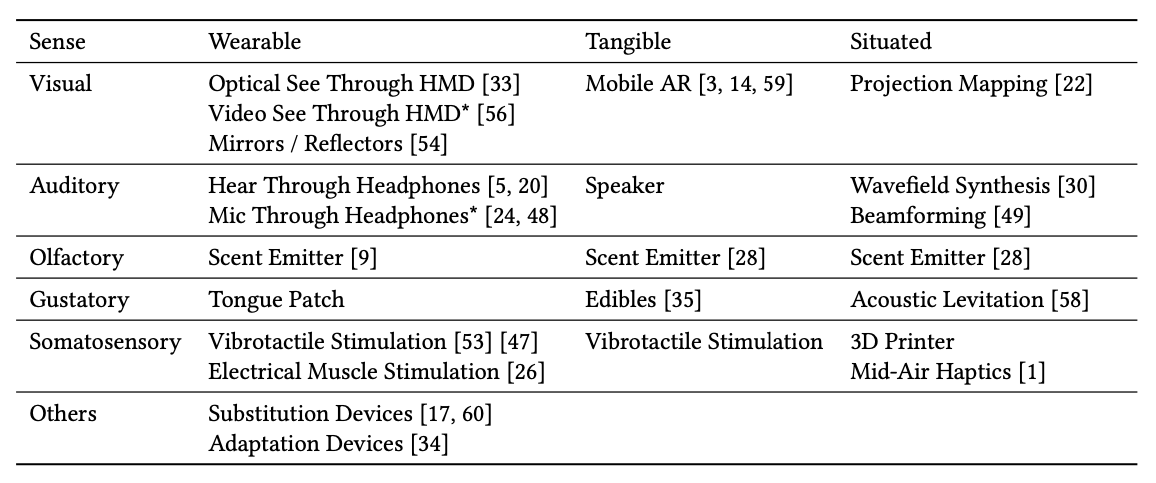
\includegraphics[width=1\linewidth]{04-method/sensorydisplays.png}}
    \caption[Potential AR Instruments, extended from \citep{lindeman2007}]{Potential AR Instruments, extended from \citep{lindeman2007}}
\end{table}\label{table: ar-instrument}

\subsubsection{Wearable}
Wearable \gls{ar} Instruments include forms that are worn on the body, including output via head-mounted visual, audio, olfactory and gustatory feedback devices or `displays', and body-mounted proprioceptive feedback devices

\subsubsection{Tangible}
Tangible \gls{ar} Instruments include forms that can explored by holding or touching, such as devices that use conductive fabrics and textiles to track input, and then providing sensory feedback, e.g. vibrotactile stimulation (somatosensory). They can also be any object that can be granted instrumentality by a device that can track it and provide contextually aware, i.e. corresponding, sensory feedback via another device. For example, a wooden cube could be transformed into a Tangible Instrument through real-time image recognition, and specific interactions with it could provide auditory feedback. In this example, the auditory feedback would likely be delivered via a Wearable Instrument that was also processing the real-time image recognition such as an \gls{hmd} with bone-conduction headphones.

\subsubsection{Situated}
Situated \gls{ar} Instruments include forms that are anchored in a real world environment and therefore provide location-specific experiences. Activation is gauged by user enaction, or user presence via infrared camera tracking or proximity of a worn device. Examples of Situated \gls{ar} Instruments could include an interactive projection mapping with wavefield synthesis providing auditory feedback, and anchored scent emitters providing olfactory feedback

\subsection{Role of the Virtual in the AR Environment}\label{sec: discussion-guidelines-environment}
\subsubsection{Allowance for the Real}
The use of the game engine Unity, and visual programming languages like \gls{pd} / Max MSP have been invaluable in the development of the three outlined sound \gls{art} experiences. Thinking about how they integrate with the real environment of your participant is how \gls{ar} stays distinct from \gls{vr} on an interaction level - after all, there must be some reason why as an artist or musician, we decide to work in tandem with, rather than shut off, the real world from our participants! Consider the following:
\begin{itemize}
    \item What are the sensory boundaries implicit in both the real and virtual space I'm using? 
    \item What different sensory affordances are provided by both the real and virtual environments? 
    \item How might the development of augmented material be influenced by the above factors?
    \item What real objects are present in the space, is this intentional?
\end{itemize}

\subsubsection{Choosing Experience Size and Complexity}
It may be helpful to distinguish between different types of \gls{ar} `experience sizes' when first starting out developing sound \gls{art}. For doing this, I developed the following three categorisations. Implying or explicitly stating these boundaries (if it is a public installation) is necessary for building trust and ensuring safety. Intentionally setting boundaries may help in the creative process too.

Snippets describe a small-scale clip-like \footnote{Similar in scale to the video-clip, sound-clip, clipart, and now app-clip, however conceptually different in that Snippets are not a miniaturised `extracts' or `segments' of a larger experience} \gls{ar} experiences that occur in the approximate interaction space of 30cm3, e.g. between a users hands. The Snippet itself does not supply a full sensorial experience, instead providing two human-to-sense interactions through its \gls{ar} subforms.

Scenes describe medium-scale \gls{ar} experiences that occur on and around the body, an approximate interaction space of 200cm3. They can be formed from existing Snippets, or created from scratch. They ideally feature more (and higher complexity) human-to-sense interactions, and therefore potentially more interactive relationships between real and virtual elements will be formed.

Spaces describe large-scale \gls{ar} experiences, involving multiple participants in a variety of differently sized interaction spaces in a room. For example, augmented hand / body interaction with the environment and other users, and multiple of zones of interaction in different sections of the space. Spaces provide fully multisensory immersive experiences, by making use of a combination of different sensory modalities and \gls{ar} subforms.

Building upon the foundation provided by these guidelines, further investigation could develop these guidelines into `design patterns', a concept from computer science that describes a set of `communicating objects and classes that are customized to solve a general design problem in a particular context' \citep{gamma1995}. A design pattern thus `names, abstracts, and identifies the key aspects of a common design structure that make it useful for creating a reusable object-oriented design'. Design patterns serve to be less rigid than frameworks, more problem-focused than guidelines; whilst inheriting the meaningful organisational structure that comes with an object-oriented design approach. Design patterns are characterised by having four elements:
\begin{itemize}
    \item The \textbf{pattern name} describes the design problem at a higher level of abstraction
    \item The \textbf{problem} describes the specific situation in which you might apply the pattern
    \item The \textbf{solution} describes the relationships between elements of the pattern that aim to solve the problem
    \item The \textbf{consequences} are the results and trade-offs of applying the pattern
\end{itemize}





